\section{Logique interne}

%%
\subsection{Nom des molécules}

Pour tracer une molécule, il suffit d'appeler \lstinline|\chemfig\{!\nomDeLaMolecule}|.
La représentation de base pour les molécules est la formule topologique, il faut ajouter un suffixe au nom pour passer à une autre représentation \important{si elle est définie, ce qui n'est pas du tout toujours le cas.} Les suffixes sont les suivants :

\begin{listePoints}[2]
  \item \lstinline{SemiDev} : formule semi-développée ;
  \item \lstinline{Dev} : formule développée ;
  \item \lstinline{Haw} : représentation de Haworth ;
  \item \lstinline{Cram} : représentation de Cram.
\end{listePoints}
Pour les acides aminés, il existe quatre autres suffixes
\begin{listePoints}[2]
  \item \lstinline{L} : représentation de Fischer gauche ;
  \item \lstinline{H} : pour tracer un polypeptide, la chaîne latérale est vers le haut ;
  \item \lstinline{D} : représentation de Fischer droite ;
  \item \lstinline{B} : pour tracer un polypeptide, la chaîne latérale est vers le bas.
\end{listePoints}

%%
\subsection{Commandes internes pour faciliter l'écriture}

Pour tracer les formules topologiques, 
j'utilise plusieurs commandes pour éviter d'avoir à spécifier en permanence les angles les plus courants
(\qty{60}{\degree}, \qty{50}{\degree}, etc.),
ou pour réutiliser des morceaux de molécules complexes

\begin{boiteCodeTex}{cote a cote = 2cm}
  \chemfig{-!\vide{::30} -} % Pour tracer une liaison invisible (utile pour les cycles incomplets)

  \chemfig{-!\vide{::-30}-}
\end{boiteCodeTex}
%
\begin{boiteCodeTex}{cote a cote = 2cm}
  \chemfig{-[:30] !\lh} % Pour tracer une liaison vers le haut (liaison haut = lh)

  \chemfig{-[:30] !\lb} % Pour tracer une liaison vers le bas (liaison bas = lb)
\end{boiteCodeTex}
%
\begin{boiteCodeTex}{cote a cote = 2cm}
  \chemfig{-[:30]!\lhb} % Pour tracer une liaison vers le haut puis vers le bas

  \chemfig{-[:30]!\lbh} % Pour tracer une liaison vers le bas puis vers le haut
\end{boiteCodeTex}
%
\begin{boiteCodeTex}{cote a cote = 2cm}
  \chemfig{-[:30]!\llh} % Pour tracer une liaison double vers le haut
  
  \chemfig{-[:30]!\llb} % Pour tracer une liaison double vers le bas
\end{boiteCodeTex}
%
\begin{boiteCodeTex}{cote a cote = 3cm}
  \chemfig{-[:-30]!\cis} % Pour tracer une liaison cis
  
  \chemfig{-[:-30]!\trans} % Pour tracer une liaison "trans" aplatie
\end{boiteCodeTex}
%
\begin{boiteCodeTex}{cote a cote = 2cm}
  \chemfig{-[:30]!\ldh} % Pour tracer une liaison développée vers le haut (l'angle est plus faible)
  
  \chemfig{-[:30]!\ldb} % Pour tracer une liaison développée vers le bas
\end{boiteCodeTex}
%
\begin{boiteCodeTex}{cote a cote = 2cm}
  \chemfig{-[:30]!\lldh} % Pour tracer une liaison double développée vers le haut
  
  \chemfig{-[:30]!\lldb} % Pour tracer une liaison double développée vers le bas
\end{boiteCodeTex}
%
\begin{boiteCodeTex}{cote a cote = 2cm}
  \chemfig[cram width = 5pt]{C !\cram{A}{B} (-[::90] R_1) -[::-30] R_2} % Pour tracer deux liaisons de cram autour d'un élément 
  
  \chemfig{-!\branche{A}{B}-} % Pour tracer deux liaisons à \qty{90}{\degree} autour d'un élément chimique
\end{boiteCodeTex}
%
\begin{boiteCodeTex}{cote a cote = 5.5cm}
  \chemfig{A- !\hexaOseHaw{!\lb B} -C} % Pour tracer des isomères du glucose
  
  \chemfig{A- !\pentaOseHaw{!\lb B}{!\lb C} -D} % Pour tracer des isomères du fructofuranose

  \chemfig{-[:30] 
    !\sterol {-A-} {-B--} {C-D-} 
      {-(-[::0] E)---} {---} {-(-[::0] F)---} 
  } % Pour tracer des stérols
\end{boiteCodeTex}

%%
\subsection{Coloriage de fonctions organiques et de parties de molécules}

\begin{boiteCodeTex}{}
\begin{tikzpicture}
  \node (base) at (0,0) {};
  \chemCarboxyle (-134pt, 14pt)
  \chemAmine (-88pt, 17pt)
  \chemAmide (71pt, 10pt)
  \node at (base) {
    \chemfig{!\alanine} $+$
    \chemfig{[:30]H_2N !\cysteineB OH} \reaction
    \chemfig{[:-30] H_2N !\alanineH !\HN !\cysteineB OH}
  };
\end{tikzpicture}
%
\begin{tikzpicture}
  \node (base) at (0,0) {};
  \chemAmide (-32pt,4pt);
  \node at (base) {\chemfig{[:-30] H_2N !\alanineH !\HN !\cysteineB OH}};
\end{tikzpicture}
%
\begin{tikzpicture}
  \node (base) at (0,0) {};
  \chemPolygone [rotation = -11] (36pt, 26pt)
  \node at (base) {\chemfig{!\adenosine}};
\end{tikzpicture}
%
\begin{tikzpicture}
  \node (base) at (0,0) {};
  \chemPolygone [rotation = 180, bords = 5] (9pt, 14pt)
  \chemPolygone [rotation = -11, couleur = couleurTer-200] (45pt, 26pt)
  \chemPentagoneHaw (-48pt,-30pt)
  \node at (base) {\chemfig{!\adenosineHaw}};
\end{tikzpicture}
%
\begin{tikzpicture}
  \node (base) at (0,0) {};
  \chemHexagoneHaw (-27pt,0pt)
  \node at (base) {\chemfig{!\glucoseHaw}};
\end{tikzpicture}
%
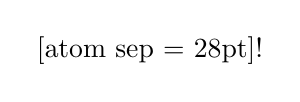
\begin{tikzpicture}
  \node (base) at (0,0) {};
  \chemHexagoneHaw[atom sep = 28pt] (-32pt,0pt)
  \node at (base) {\chemfig[atom sep = 28pt]{!\glucoseHaw}};
\end{tikzpicture}
\end{boiteCodeTex}
